\documentclass[11pt]{article}

\usepackage[a4paper,margin=1in]{geometry}
\usepackage[T1]{fontenc}
\usepackage[utf8]{inputenc}
\usepackage{lmodern}
\usepackage{microtype}
\usepackage{amsmath,amssymb,amsthm,mathtools}
\usepackage{booktabs,array,graphicx,float}
\usepackage[section]{placeins}
\usepackage{enumitem}
\usepackage[numbers,sort&compress]{natbib}
\usepackage{xcolor,xurl}
\usepackage[colorlinks=true,linkcolor=blue!55!black,citecolor=blue!55!black,urlcolor=blue!55!black]{hyperref}
\usepackage[nameinlink,noabbrev]{cleveref}

\setlength{\parindent}{1.4em}
\setlength{\parskip}{0.12em}
\setlist{itemsep=0.25em,topsep=0.35em}

\newtheorem{theorem}{Theorem}[section]
\newtheorem{proposition}[theorem]{Proposition}
\newtheorem{corollary}[theorem]{Corollary}
\theoremstyle{definition}
\newtheorem{definition}[theorem]{Definition}
\theoremstyle{remark}
\newtheorem{remark}[theorem]{Remark}

\newcommand{\C}{\mathbb C}
\newcommand{\Id}{\mathrm I}
\newcommand{\cD}{\mathcal D}
\newcommand{\cE}{\mathcal E}
\newcommand{\cK}{\mathcal K}
\newcommand{\HS}{\mathfrak S_2}
\newcommand{\tr}{\operatorname{tr}}
\newcommand{\spr}{\operatorname{spr}}
\newcommand{\Ran}{\operatorname{Ran}}
\newcommand{\rank}{\operatorname{rank}}
\newcommand{\Ker}{\operatorname{Ker}}
\newcommand{\norm}[1]{\left\lVert #1\right\rVert}

\title{Cyclic-Rank Obstructions and Growing-Horizon Stein Certificates\\
\large Minimal Gramians, Conic No-Go Witnesses, and a Viable Block Route}
\author{Liang Wang}
\date{July 2026}

\begin{document}
\maketitle

\begin{abstract}
The preceding two-pole Hardy reduction converted the remaining
small-noise range-resolvent gate for the folded-Gaussian quadratic operator
into positive Stein inequalities.  We determine what an exact positive
certificate can and cannot look like.  For a stable scaled bulk matrix
\(A=N/r\), a directional source \(X\), and
\[
 G=\sum_{m\ge0}A^mXX^*(A^*)^m,
 \qquad G-AGA^*=XX^*,
\]
we prove that \(G\) is the minimal positive Stein supersolution and that
\[
 \Ran G=\operatorname{span}\{A^m\Ran X:m\ge0\}.
\]
Every positive supersolution has an \(A\)-invariant range containing this
cyclic subspace, hence rank at least \(\rank G\).  Fixed-rank exact
Lyapunov factors are therefore impossible whenever the directional cyclic
dimension grows.  If \(H=ZZ^*+\alpha\Id\ge G\) and \(\rank Z\le k\),
then necessarily \(\alpha\ge\lambda_{k+1}(G)\).

The obstruction does not close the Stein route.  With
\[
 S_M=\sum_{j=0}^{M-1}A^jXX^*(A^*)^j,
\]
the block inequality \(H-A^MH(A^*)^M\ge S_M\) already implies \(H\ge G\).
If \(q_M=\norm{A^M}<1\), then
\[
 H_M=S_M+\alpha_M\Id,
 \qquad
 \alpha_M=\frac{\norm{A^MS_M(A^*)^M}}{1-q_M^2}
\]
is an explicit block supersolution.  Thus the fixed-step
global-contraction no-go of the preceding paper is compatible with a
horizon increasing with noise resolution.  We also give an anisotropic
residual completion and conic dual witnesses that rule out whole metric
ansatz classes.

A five-scale binary64 dense audit, with \(N\sigma=5.12\), \(r=0.85\), and
\(N=32,\ldots,512\), solves both directional Gramians.  The left and right
energies remain between \(0.904\)--\(1.468\) and \(1.003\)--\(1.760\),
while the ranks carrying \(99\%\) of the Gramian trace grow from \(5\) to
\(69\) and from \(5\) to \(64\).  At relative singular threshold
\(10^{-8}\), the left cyclic rank grows from \(22\) to \(322\), about
\(0.63N\) at the finest scale.  Scalar identity metrics have rank-one dual
obstructions at the four finest levels, and the diagonal extracted from
the exact Gramian fails at all five.  In contrast, block horizons
\(4,8,16,24,32\) give energy uppers within \(6.3\times10^{-4}\) relative
of the dense Gramian energies.  These are floating diagnostics, not a
dyadically uniform theorem.  No arithmetic trace formula, zeta-zero
identity, self-adjoint realization, or Riemann-hypothesis conclusion is
claimed.
\end{abstract}

\noindent\textbf{Keywords:} Stein inequality; controllability Gramian;
cyclic subspace; Lyapunov rank; block certificate; conic duality;
small-noise transfer operator; Hardy energy.

\medskip
\noindent\textbf{MSC 2020:} 47A10; 93B05; 93B36; 15A24; 65F45.

\section{Introduction}

RH-50 reduced the two Hilbert--Schmidt range-resolvent actions left by
RH-49 to directional Hardy energies and positive Stein inequalities
\citep{WangDirectional2026,WangHardy2026}.  This turns a contour problem
into an infinite time-domain energy, but it also raises a structural
question: can an exact certificate be low rank, scalar, diagonal, or based
on a fixed number of noisy steps?

Large-scale Lyapunov solvers often provide accurate low-rank approximations
\citep{Antoulas2005,BennerLiPenzl2008,Simoncini2016}.  Accuracy, however,
is not the same as a positive Loewner certificate.  Exact domination
remembers the complete directional cyclic subspace.  We first prove the
resulting rank obstruction, then show that it does not force a global
inverse or fixed-step contraction.  Grouping time into blocks permits a
horizon \(M=M(\sigma,n)\) that grows with the mixing scale.  A finite
Krylov sum plus a positive tail background then gives a complete
certificate.

The numerical outcome is a route selection.  The exact finite Gramians
become increasingly high-dimensional even though their observed Hardy
energies remain moderate.  Fixed-rank and scalar shortcuts are therefore
poor targets.  A growing-horizon block certificate, on the other hand, is
extremely sharp on every stored scale.

\section{The two directional Hardy pairs}

Let \(T=G_{2n,\sigma}\) be the fine folded-Gaussian Galerkin matrix and let
\(A_c=G_{n,\sigma}\) be its exact coarse Haar block.  Relative to the
adjacent Haar split,
\[
 T=\begin{pmatrix}A_c&B\\C&D\end{pmatrix}.
\]
Remove the fine and coarse Perron/parity channels:
\begin{align*}
 Q_f&=\Id-P_{f,+}-P_{f,-},
 &N_f&=T-P_{f,+}-\lambda_{f,-}P_{f,-},\\
 Q_c&=\Id-P_{c,+}-P_{c,-},
 &N_c&=A_c-P_{c,+}-\lambda_{c,-}P_{c,-}.
\end{align*}
Let \(U\) be the isometric coarse-to-fine embedding and let \(r\) exceed
both bulk spectral radii.  Define
\begin{align}
 A_B&=r^{-1}N_f,
 &X_B&=\frac{Q_fUB}{\norm B_{\HS}},
 &Y_B&=U^*, \label{eq:left-pair}\\
 A_C&=r^{-1}N_c^*,
 &X_C&=\frac{C^*}{\norm C_{\HS}},
 &Y_C&=Q_c^*. \label{eq:right-pair}
\end{align}
For \(s\in\{B,C\}\), put
\[
 G_s=\sum_{m\ge0}A_s^mX_sX_s^*(A_s^*)^m.
\]
Cyclicity of the finite trace gives
\begin{equation}
 \cE_B(r)^2=\tr(Y_BG_BY_B^*),
 \qquad
 \cE_C(r)^2=\tr(Y_CG_CY_C^*).
 \label{eq:energy-traces}
\end{equation}
Thus both RH-50 energies have the same abstract form.  We now work with a
generic stable pair \((A,X)\).

\section{Minimality, cyclic support, and rank}

Let \(A\in\C^{d\times d}\), \(\spr(A)<1\), and
\(X\in\C^{d\times p}\).  Define
\begin{equation}
 G=\sum_{m=0}^{\infty}A^mXX^*(A^*)^m,
 \qquad
 \cK(A,X)=\operatorname{span}\{A^m\Ran X:m\ge0\}.
 \label{eq:G-K}
\end{equation}
By Cayley--Hamilton, powers through \(d-1\) suffice in the second formula.

\begin{theorem}[Minimal Gramian and cyclic support]
\label{thm:minimal}
The matrix \(G\) is the unique Hermitian solution of
\[
 G-AGA^*=XX^*.
\]
If \(H\ge0\) and
\begin{equation}
 H-AHA^*\ge XX^*,
 \label{eq:one-step}
\end{equation}
then
\begin{equation}
 H\ge G,
 \qquad
 \Ran G=\cK(A,X),
 \qquad
 \Ran X\subseteq\Ran H,
 \qquad
 A\Ran H\subseteq\Ran H.
 \label{eq:minimal-range}
\end{equation}
Consequently
\begin{equation}
 \boxed{\rank H\ge\dim\cK(A,X)=\rank G.}
 \label{eq:rank-lower}
\end{equation}
\end{theorem}

\begin{proof}
Separating the first term of the convergent series gives the Stein
equality.  If two Hermitian solutions differ by \(D=ADA^*\), then
\(D=A^mD(A^*)^m\to0\), so the solution is unique
\citep{ZhouDoyleGlover1996,HornJohnson2013}.

Iterating \eqref{eq:one-step} gives
\[
 H\ge\sum_{m=0}^{M-1}A^mXX^*(A^*)^m+A^MH(A^*)^M.
\]
Discard the positive remainder and let \(M\to\infty\), obtaining \(H\ge G\).
Moreover,
\[
 v^*Gv=\sum_{m\ge0}\norm{X^*(A^*)^mv}^2,
\]
so \(\Ker G=\cK(A,X)^\perp\), which proves the range identity.

The inequality \(H\ge XX^*\) implies
\(\Ker H\subseteq\Ker X^*\), hence \(\Ran X\subseteq\Ran H\).  Also
\(H\ge AHA^*\).  If \(v\in\Ker H\), then
\[
 0\le v^*AHA^*v\le v^*Hv=0,
\]
so \(A^*v\in\Ker H\).  Hence \(\Ran H\) is \(A\)-invariant and contains
the smallest invariant subspace generated by \(X\).  This proves
\eqref{eq:rank-lower}.
\end{proof}

\begin{corollary}[Fixed-rank exact-certificate no-go]
If \(\dim\cK(A_\nu,X_\nu)\to\infty\) along a family, no exact positive
Stein supersolution family can have uniformly bounded rank.
\end{corollary}

\begin{remark}
Low-rank Krylov or ADI factors may still approximate \(G\) very accurately.
The theorem says that once a cyclic direction is omitted, the factor alone
cannot be an exact positive certificate.  A positive background completion
remains possible.
\end{remark}

\section{The unavoidable background floor}

Write
\(\lambda_1(G)\ge\cdots\ge\lambda_d(G)\ge0\).

\begin{theorem}[Low-rank plus isotropic floor]
\label{thm:floor}
If
\[
 H=ZZ^*+\alpha\Id\ge G,
 \qquad
 \rank Z\le k<d,
 \qquad
 \alpha\ge0,
\]
then
\begin{equation}
 \boxed{\alpha\ge\lambda_{k+1}(G).}
 \label{eq:floor}
\end{equation}
\end{theorem}

\begin{proof}
Loewner monotonicity and the min--max principle give
\(\lambda_{k+1}(G)\le\lambda_{k+1}(H)\).  Since \(ZZ^*\) has rank at most
\(k\), at most \(k\) eigenvalues of \(H\) exceed \(\alpha\), and
\(\lambda_{k+1}(H)=\alpha\) \citep{HornJohnson2013}.
\end{proof}

For an observation \(Y\),
\begin{equation}
 \tr(YHY^*)=\norm{YZ}_{\HS}^2+\alpha\norm Y_{\HS}^2.
 \label{eq:floor-cost}
\end{equation}
In the left pair, \(Y_B=U^*\) and \(\norm{Y_B}_{\HS}^2=n\).
Therefore even a small scalar floor may have a dimensional trace cost.
This is why an anisotropic background is eventually preferable.

\section{Growing-horizon block certificates}

For \(M\ge1\), put
\begin{equation}
 S_M=\sum_{j=0}^{M-1}A^jXX^*(A^*)^j,
 \qquad
 \cD_M(H)=H-A^MH(A^*)^M.
 \label{eq:block-definitions}
\end{equation}

\begin{theorem}[Block Stein domination]
\label{thm:block}
If \(H\ge0\) and
\begin{equation}
 \cD_M(H)\ge S_M,
 \label{eq:block-super}
\end{equation}
then \(H\ge G\).  The exact Gramian satisfies
\(\cD_M(G)=S_M\) for every \(M\).  Every one-step supersolution satisfies
\eqref{eq:block-super} for every \(M\).
\end{theorem}

\begin{proof}
Iterating \eqref{eq:block-super} over \(L\) blocks yields
\[
 H\ge
 \sum_{k=0}^{L-1}A^{kM}S_M(A^*)^{kM}
 +A^{LM}H(A^*)^{LM}
 =
 \sum_{m=0}^{LM-1}A^mXX^*(A^*)^m
 +A^{LM}H(A^*)^{LM}.
\]
Discard the final positive term and let \(L\to\infty\).  Grouping the
series for \(G\) proves equality.  Finally,
\[
 H-A^MH(A^*)^M
 =\sum_{j=0}^{M-1}A^j(H-AHA^*)(A^*)^j,
\]
which proves the last statement.
\end{proof}

The block theorem is not a rank loophole: every block supersolution still
dominates \(G\).  Its advantage is temporal.  Positivity may become easy
only after a horizon that increases with the noise-dependent mixing time.

\begin{theorem}[Finite Krylov sum plus isotropic tail]
\label{thm:isotropic}
Let \(P_M=A^M\), \(q_M=\norm{P_M}<1\), and define
\begin{equation}
 R_M=P_MS_MP_M^*,
 \qquad
 \alpha_M=\frac{\norm{R_M}}{1-q_M^2},
 \qquad
 H_M=S_M+\alpha_M\Id.
 \label{eq:HM}
\end{equation}
Then \(\cD_M(H_M)\ge S_M\), hence \(H_M\ge G\).  For every observation
\(Y\),
\begin{equation}
 \boxed{
 \tr(YGY^*)
 \le
 \tr(YS_MY^*)
 +\frac{\norm{P_MS_MP_M^*}}{1-q_M^2}\norm Y_{\HS}^2.}
 \label{eq:block-energy}
\end{equation}
Moreover
\[
 \alpha_M\le\frac{q_M^2\norm{S_M}}{1-q_M^2}.
\]
\end{theorem}

\begin{proof}
Since
\(\Id-P_MP_M^*\ge(1-q_M^2)\Id\) and
\(\norm{R_M}\Id\ge R_M\),
\[
 \cD_M(H_M)-S_M
 =
 \alpha_M(\Id-P_MP_M^*)-R_M\ge0.
\]
Apply \cref{thm:block}, pair \(H_M\ge G\) with \(Y^*Y\), and use
\(\norm{R_M}\le q_M^2\norm{S_M}\).
\end{proof}

If \(\norm Y_{\HS}^2\asymp n\), the isotropic tail is controlled once
\(q_M=O(n^{-1/2})\), provided the finite-horizon quantities are bounded.
Exponential decay after a transient would make this a logarithmic horizon
\(M=O(\log n)\).  RH-50 rules out a noise-uniform fixed \(M\); it does not
rule out \(M=M(\sigma,n)\to\infty\).

\section{Anisotropic completion and conic witnesses}

The identity floor is universal but may be expensive.  The next theorem
isolates what a structured positive background must prove.

\begin{theorem}[Residual/background completion]
\label{thm:background}
Let \(\widehat H\ge0\), \(W\ge0\), and
\[
 E_M=S_M-\cD_M(\widehat H).
\]
If \(\cD_M(W)\ge\mu\Id\) for some \(\mu>0\), then
\[
 H=\widehat H+\alpha W,
 \qquad
 \alpha\ge
 \frac{\max\{0,\lambda_{\max}(E_M)\}}{\mu}
\]
is a block supersolution and dominates \(G\).
\end{theorem}

\begin{proof}
Directly,
\[
 \cD_M(H)-S_M
 =\alpha\cD_M(W)-E_M
 \ge\alpha\mu\Id-E_M\ge0.
\]
Apply \cref{thm:block}.
\end{proof}

Here \(\widehat H\) may be a truncated Krylov factor, banded matrix, or
multilevel sum.  The background \(W\) may weight only the sectors carrying
the residual, replacing the cost \(\alpha\norm Y_{\HS}^2\) by
\(\alpha\tr(YWY^*)\).

\begin{theorem}[Positive conic dual witness]
\label{thm:conic}
Let \(W_1,\ldots,W_J\ge0\).  Suppose \(Z\ge0\) satisfies
\[
 \tr\!\left(Z(W_j-AW_jA^*)\right)\le0
 \quad(j=1,\ldots,J),
 \qquad
 \tr(ZXX^*)>0.
\]
Then no nonnegative conic combination
\[
 H=\sum_{j=1}^Jh_jW_j,
 \qquad h_j\ge0,
\]
satisfies \(H-AHA^*\ge XX^*\).
\end{theorem}

\begin{proof}
If it did, positivity would give
\[
 0\le
 \tr\!\left(Z(H-AHA^*-XX^*)\right)
 =
 \sum_jh_j\tr\!\left(Z(W_j-AW_jA^*)\right)-\tr(ZXX^*)<0,
\]
a contradiction.
\end{proof}

Taking \(Z=vv^*\) gives the cheap rank-one test
\[
 v^*(W_j-AW_jA^*)v\le0\quad\text{for every }j,
 \qquad
 \norm{X^*v}^2>0.
\]
The same theorem holds for block defects with source \(S_M\).

\section{Five-scale dense Gramian audit}

The experiment uses the row-normalized folded-Gaussian matrices of RH-50
at the smaller dense-solve resolution
\[
 N\sigma=5.12,
 \qquad r=0.85.
\]
Both peripheral channels are removed with dense binary64 eigendata.  The
complete finite Lyapunov equations are then solved through \(N=512\).
Here \emph{exact Gramian} means the complete dense finite-matrix solution,
not exact arithmetic or interval validation.

For a positive Gramian define
\[
 r_{\mathrm{eff}}(G)=\frac{(\tr G)^2}{\tr(G^2)},
\]
and let \(r_{99}\) be the least rank carrying \(99\%\) of the trace.  The
cyclic ranks below are numerical ranks of
\([X,AX,\ldots,A^9X]\) at relative singular threshold \(10^{-8}\).

\begin{table}[H]
\centering
\small
\begin{tabular}{@{}rrrrrrrrr@{}}
\toprule
\(\sigma\)&\(N\)&\(\cE_B\)&\(\cE_C\)&\(r_{\rm eff}^B\)&\(r_{99}^B\)&\(r_{\rm eff}^C\)&\(r_{99}^C\)&cyclic\\
\midrule
0.16&32 &0.9040&1.0026&2.40 &5 &2.82 &5 &22\\
0.08&64 &1.1626&1.2653&5.09 &9 &5.54 &9 &43\\
0.04&128&1.3338&1.4845&8.62 &17&8.42 &17&84\\
0.02&256&1.4096&1.6340&15.51&35&12.33&33&165\\
0.01&512&1.4681&1.7603&25.66&69&16.30&64&322\\
\bottomrule
\end{tabular}
\caption{Dense five-scale Gramian audit.  Energies use complete binary64
Lyapunov solutions.  The ranks are diagnostics, not validated asymptotic
lower bounds.}
\label{tab:gramian}
\end{table}

The energies remain moderate, but state complexity grows rapidly.  The
left and right \(99\%\) ranks are
\[
 (5,9,17,35,69),
 \qquad
 (5,9,17,33,64),
\]
with fitted dimension powers \(0.9533\) and \(0.9231\).  The terminal
cyclic ranks
\[
 (22,43,84,165,322)
\]
have fitted power \(0.9683\) and maximum log residual \(0.0021\).  At the
finest scale the thresholded cyclic span occupies \(62.9\%\) of the state
dimension.  This is strong evidence against a fixed-rank physical
certificate, but a rigorous physical asymptotic no-go still requires an
analytic cyclic-dimension lower bound.

\subsection{Simple metrics}

For the left pair, the minimum eigenvalues of the unforced identity defects
\(\Id-A_BA_B^*\) are
\[
 0.5064,\quad -0.2002,\quad -1.1961,\quad -2.5744,\quad -4.5093.
\]
At the four finest levels, a minimum-eigenvector also has positive source
overlap.  By \cref{thm:conic}, no scalar multiple \(h\Id\), \(h\ge0\), is
a Stein supersolution there.

Simply extracting the diagonal of the exact Gramian also fails.  The
minimum eigenvalues of
\[
 \widehat G-A_B\widehat G A_B^*-X_BX_B^*,
 \qquad
 \widehat G=\operatorname{diag}(G_B),
\]
are
\[
 -0.3545,\quad -0.2874,\quad -0.2213,\quad -0.1675,\quad -0.1232.
\]
This does not rule out an independently optimized diagonal metric, much
less a banded or multilevel metric.

\subsection{Growing horizons}

The experiment checks
\[
 M\in\{1,2,4,8,12,16,24,32,48,64\}
\]
and selects the first checkpoint for which
\[
 \norm{A^M}^2\norm Y_{\HS}^2\le0.25.
\]
It then constructs \(H_M\) from \cref{thm:isotropic}.

\begin{table}[H]
\centering
\small
\begin{tabular}{@{}rrrrrrrr@{}}
\toprule
\(\sigma\)&\(N\)&\(M\)&\(q_M^B\)&\(q_M^C\)&left exact/upper&right exact/upper&max excess\\
\midrule
0.16&32 &4 &0.0210&0.0198&0.9040/0.9042&1.0026/1.0029&\(3.1\times10^{-4}\)\\
0.08&64 &8 &0.0305&0.0279&1.1626/1.1632&1.2653/1.2661&\(6.3\times10^{-4}\)\\
0.04&128&16&0.0156&0.0156&1.3338/1.3340&1.4845/1.4850&\(3.5\times10^{-4}\)\\
0.02&256&24&0.0133&0.0124&1.4096/1.4097&1.6340/1.6344&\(2.6\times10^{-4}\)\\
0.01&512&32&0.0069&0.0067&1.4681/1.4681&1.7603/1.7604&\(6.7\times10^{-5}\)\\
\bottomrule
\end{tabular}
\caption{Growing-horizon isotropic block completions.  The defects are
positive to binary64 precision, not interval-certified.}
\label{tab:block}
\end{table}

The selected horizons are
\[
 4,\quad8,\quad16,\quad24,\quad32.
\]
A linear fit against \(\log_2N\) has slope \(7.2\), intercept \(-33.6\),
and maximum residual \(1.6\).  This is only logarithmic-looking finite
evidence, but it is the behavior required by the block route.  The largest
relative energy excess is \(5.45\times10^{-4}\) on the left and
\(6.28\times10^{-4}\) on the right.  The smallest binary64 block-defect
eigenvalue is \(1.34\times10^{-13}\), so an eventual computer-assisted
proof must use outward rounding.

\begin{figure}[H]
\centering
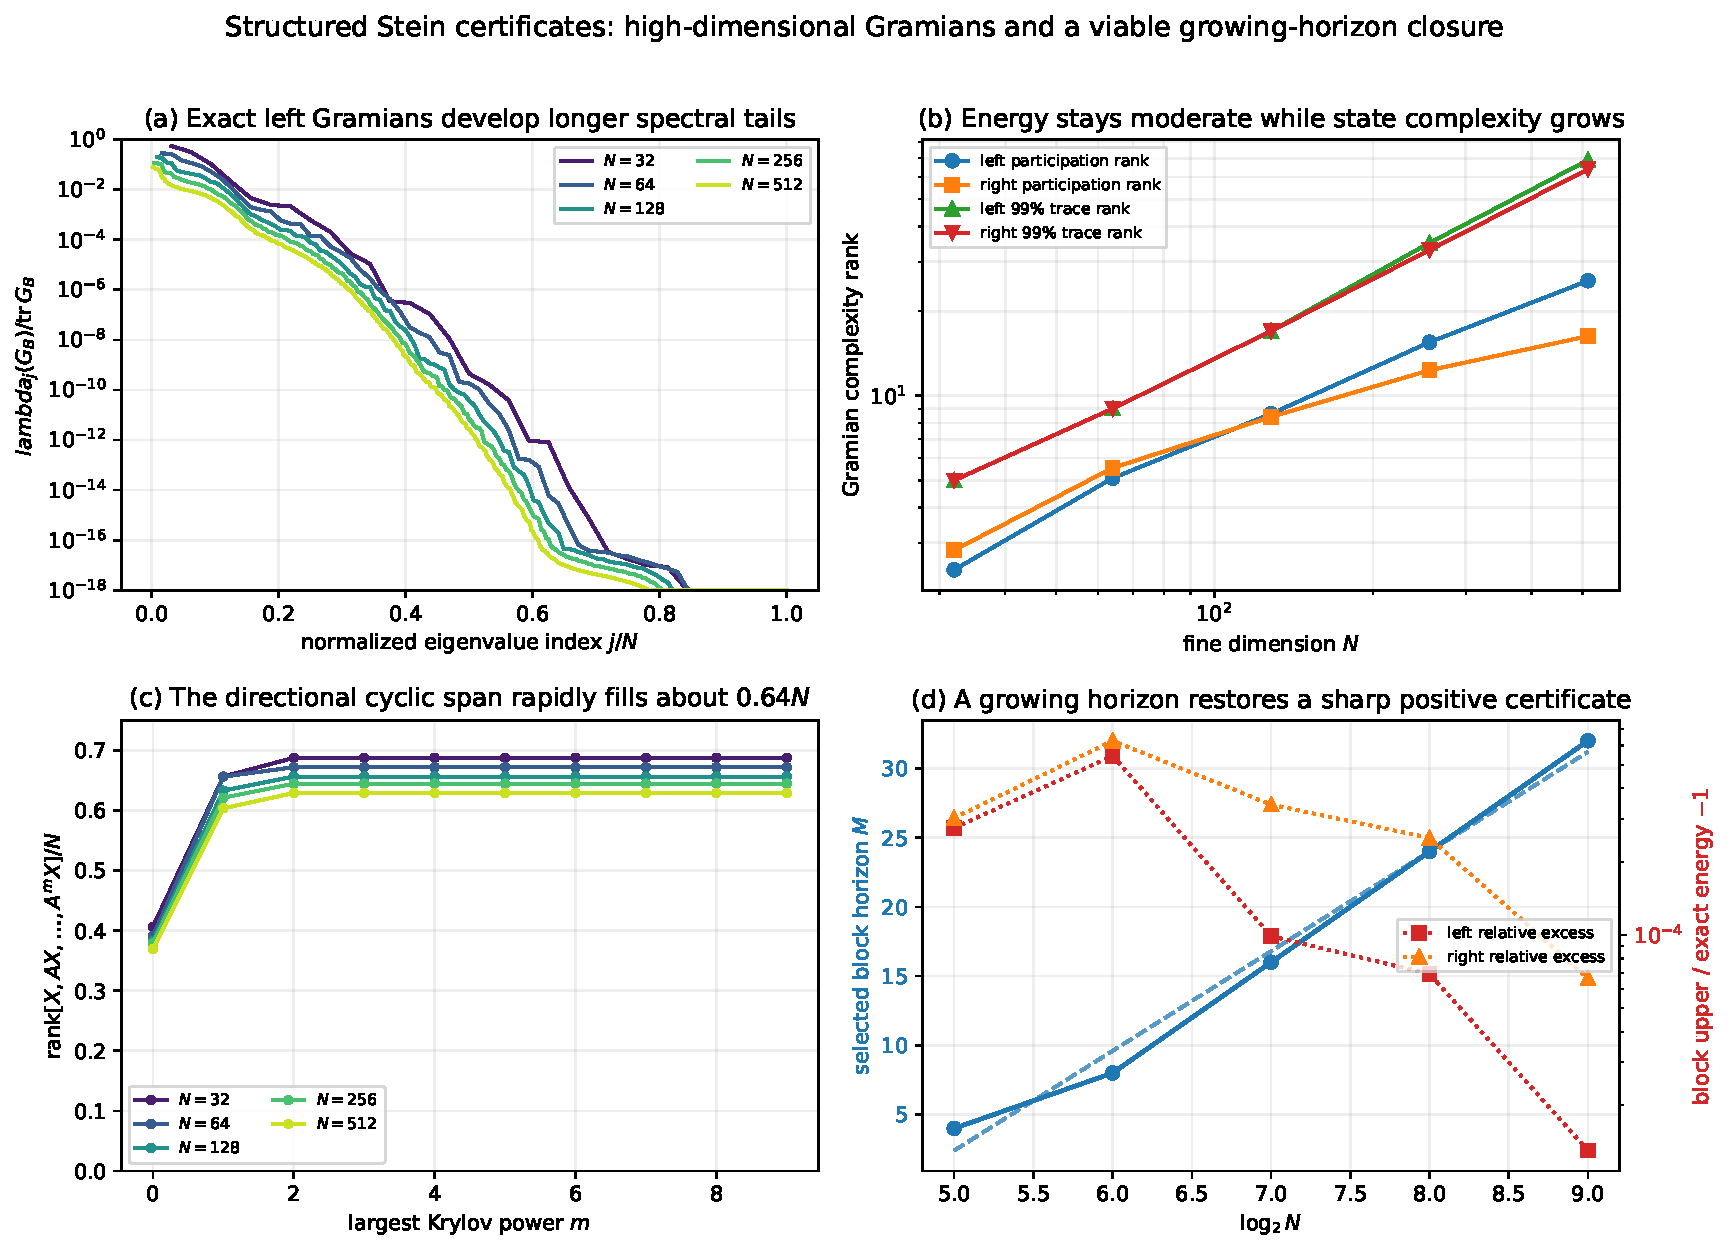
\includegraphics[width=\textwidth]{figures/structured_stein_geometry.pdf}
\caption{Five-scale audit.  (a) The normalized left Gramian spectra develop
longer tails.  (b) Effective and \(99\%\) ranks grow with dimension.
(c) The thresholded cyclic span rapidly fills about \(0.64N\).
(d) A growing horizon gives block energy uppers within
\(6.3\times10^{-4}\) relative of the dense Gramians.}
\label{fig:geometry}
\end{figure}

\section{Roadmap consequence and theorem boundary}

RH-51 closes several shortcuts and leaves one viable route
\citep{WangRoadmap2026}.

\begin{description}[leftmargin=4.4cm,style=nextline]
 \item[Fixed-rank exact factors]
 Impossible unless the directional cyclic dimension stays uniformly
 bounded.  The physical audit strongly points in the opposite direction.

 \item[Scalar identity and extracted diagonal]
 The identity cone is obstructed at the four finest stored levels, and the
 diagonal of the exact Gramian fails at all five.

 \item[Growing-horizon block route]
 Viable and numerically sharp.  The fixed-step no-go is not a no-go for
 \(M=M(\sigma,n)\).

 \item[Stage A1]
 Not closed.  The missing theorem is a dyadically uniform analytic trace
 budget for an anisotropic or multilevel growing-horizon completion.
\end{description}

The next constructive ansatz should combine a finite Krylov transport part,
a positive endpoint/interior multilevel background, and an a posteriori
residual bound.  Candidate cones should first be screened by
\cref{thm:conic}.  The scheduled RH-52 peripheral-factor transfer can
proceed independently, but the RH-54 intrinsic-identification synthesis
still requires this A1 trace budget.

The TPC series remains an independent twin-prime and prime-correlation
program.  Its methods may be referenced, but it is not an assumption or
the arithmetic half of this RH result.  We do not construct a prime-power
trace formula, identify a zeta zero, build a self-adjoint Hilbert--P\'olya
operator, derive a \(T\log T\) counting law, prove the Riemann hypothesis,
or prove a twin-prime statement.

\section{Reproducibility}

The archive contains the algebra in \path{src/structured_stein}, the
five-scale pilot and certificate builders in \path{experiments}, the figure,
tests, result ledgers, dependency hashes, summary, and archive verification.
The principal commands are
\begin{verbatim}
PYTHONDONTWRITEBYTECODE=1 /root/math/.venv/bin/pytest -q
OPENBLAS_NUM_THREADS=16 OMP_NUM_THREADS=16 \
PYTHONDONTWRITEBYTECODE=1 /root/math/.venv/bin/python \
  experiments/run_structured_stein_pilot.py
PYTHONDONTWRITEBYTECODE=1 /root/math/.venv/bin/python \
  experiments/build_stein_certificate.py
MPLBACKEND=Agg PYTHONDONTWRITEBYTECODE=1 /root/math/.venv/bin/python \
  experiments/make_figures.py
latexmk -pdf -interaction=nonstopmode -halt-on-error main.tex
PYTHONDONTWRITEBYTECODE=1 /root/math/.venv/bin/python \
  experiments/build_archive.py
PYTHONDONTWRITEBYTECODE=1 /root/math/.venv/bin/python \
  experiments/verify_archive.py
\end{verbatim}

The minimality, cyclic-support, rank, floor, block, residual-completion,
and conic-witness statements are rigorous finite-dimensional theorems.
The physical rank growth, logarithmic-looking horizon, simple-metric
failures, and near-exact block uppers are binary64 diagnostics at
\(N\sigma=5.12\).  They are not interval enclosures and do not prove a
uniform small-noise Hardy bound.

\bibliographystyle{plainnat}
\bibliography{references}

\end{document}
